\section{Design}

\subsection{Overview}
\begin{figure*}[htbp]
	\centering
	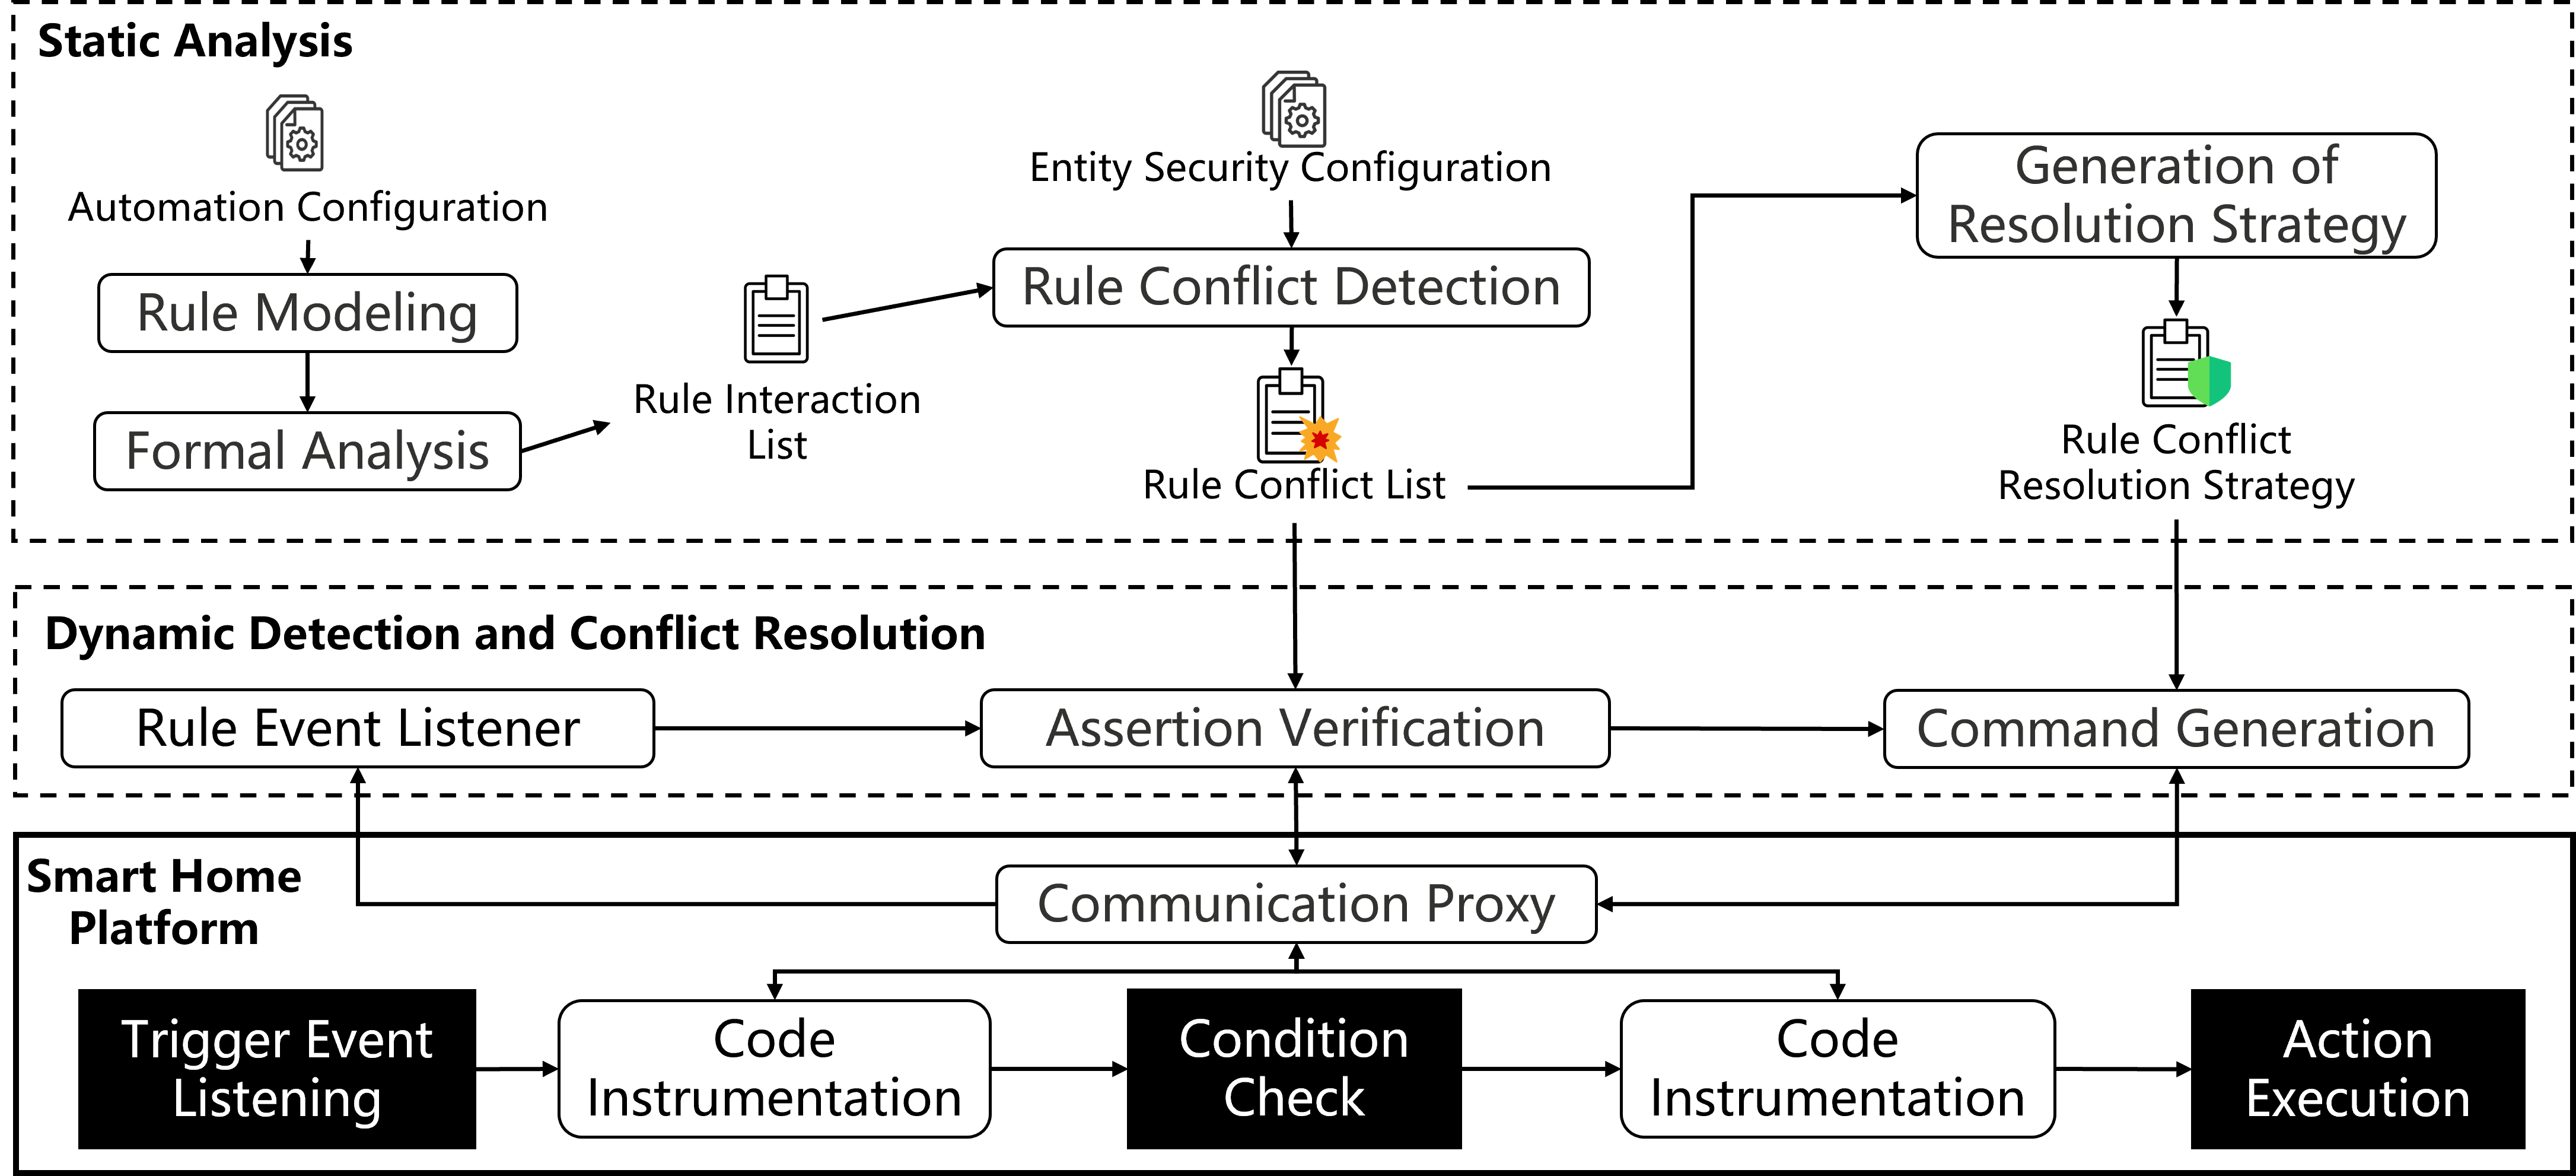
\includegraphics[width=\textwidth]{figure/overall_design.png}
	\caption{Overall Architecture of Our Approach}
	\label{overall_design}
\end{figure*}
%我们设计了一个完整的系统用于采用静态与动态结合的方式检测隐含在规则交互中的规则冲突,并且在规则冲突发生之前自动执行定制化的冲突处理策略,避免规则冲突的真实发生,并且支持。根据图片Fig.\ref{overalldesign},我们的方法主要包括两个步骤:1) 静态分析;2) 动态检测和冲突处理。
A complete system is designed that detects rule conflicts hidden in rule interactions by combining static and dynamic approaches, and automatically executes customized conflict resolution strategies before conflicts occur to prevent actual conflicts. According to Fig.\ref{overall_design}, our method mainly includes two steps: 1) Static analysis; 2) Dynamic detection and conflict resolution.

%在第一个步骤中包含了规则建模模块、形式化分析模块、静态规则冲突检测模块与冲突处理策略生成模块。智能家居系统中的自动化规则将被重新建模以实现对家庭环境区域的区分。之后,形式化分析将基于新的规则模型,从而提取所有类型的规则交互与对应的规则交互分析数据。用户的实体安全配置将被应用于规则冲突检测模块,用于将规则冲突从规则交互集合中提取出来。考虑到一个规则交互是否属于规则冲突的定义比较主观,我们提供用户配置接口,其中形式化分析模块提取的规则交互分析数据将会以自然语言形式展示给用户,以辅助用户完成对于规则冲突的判断。最终规则冲突处理策略生成模块将会为形成的规则冲突集合中的每个元素生成定制化的规则冲突处理策略。
The first step includes a rule modeling module, a formal analysis module, a static rule conflict detection module, and a resolution strategy generation module. The rules in the smart home system will be remodeled to achieve differentiation of environment zones. Afterwards, formal analysis will be based on the new rule model to extract all types of rule interactions along with corresponding rule interaction analysis data. The entity security configuration will be applied to the rule conflict detection module to extract rule conflicts from the set of rule interactions. Considering that the definition of whether a rule interaction constitutes a rule conflict is relatively subjective, system provides a user configuration interface through which the rule interaction analysis data extracted by formal analysis module will be displayed to the user in natural language to assist the user in determining rule conflicts. Finally, for each element in the formed set of rule conflicts, the resolution strategy generation module will generate a customized rule conflict resolution strategy.

%在第二个步骤中包含了规则事件监听模块,断言验证模块与命令生成模块,除此之外智能家居系统(这里使用的是Home Assistant)中的代码插装模块将会辅助完成动态的规则冲突检测与规则冲突预防。规则监听模块将会实时监听规则执行信息,当有规则一条规则在被触发,在条件检查前后时机,会将相关信息发送给断言检测模块。断言检测模块将会根据过去规则执行事件与当前正在执行的规则信息、相关设备状态信息进行断言检测,判断规则冲突是否真实发生。如果是,则命令生成模块将会根据当前即将发生的规则冲突信息,根据静态检测中的规则冲突处理策略生成执行命令,交由代码插装模块强制执行。
In the second step, a rule event listener module, an assertion verification module, and a command generation module are included. In addition, the code instrumentation module in the smart home system for example Home Assistant will assist in dynamic rule conflict detection and prevention. The rule event listener module will monitor rule execution information in real time. When a rule is triggered, before and after condition checking, it will send the relevant information to the assertion checking module. The assertion check module will then perform assertion checks based on historical rule execution events, the information of the currently executing rule, and related device status information, to determine whether a rule conflict has actually occurred. If so, the command generation module will generate execution commands based on the current rule conflict information about to occur and the rule conflict resolution strategy from static detection, which will be enforced by the code instrumentation module.

\subsection{Static Phase}

\subsubsection{Rule Modeling}

%\begin{figure}[htbp]
%	\centering
%	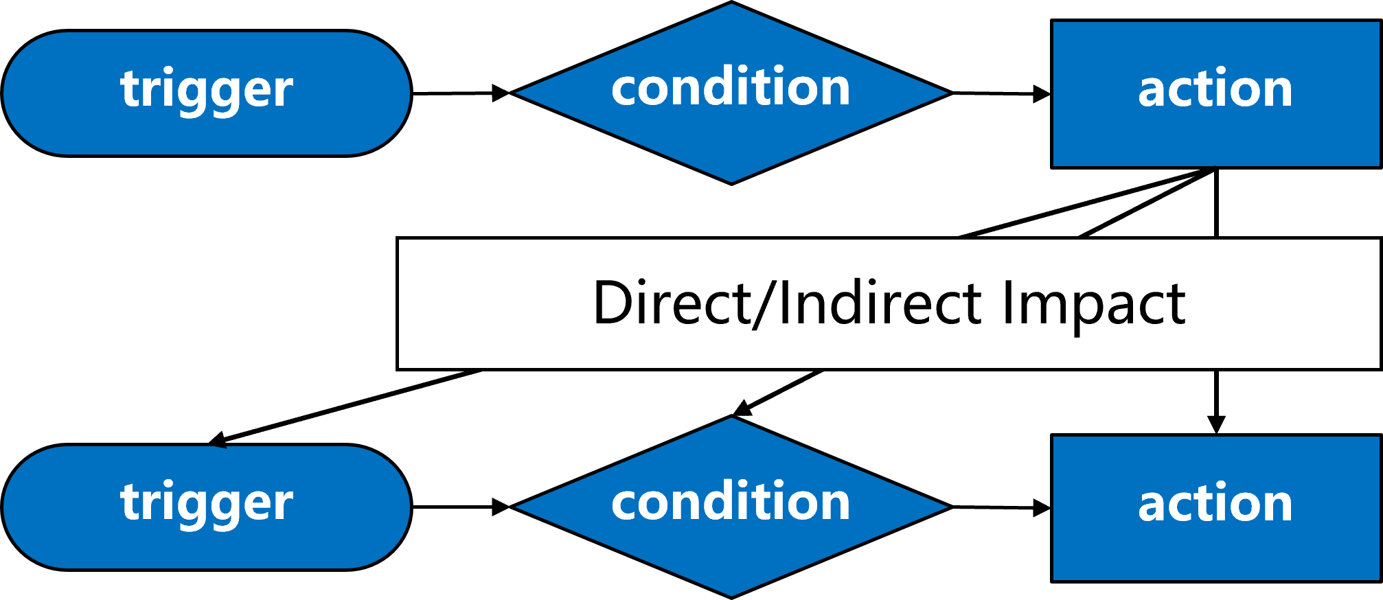
\includegraphics[width=0.4\textwidth]{figure/classification_observation.png}
%	\caption{Rule Interaction Pattern}
%	\label{classification_observation}
%\end{figure}

%在正式介绍静态步骤之前,需要介绍一下本方案对规则交互与规则冲突的分类。根据之前的观察我们将规则之间的交互使用以下方法归纳:一条规则的执行结果对零一条规则的触发器、条件与动作产生直接与间接影响。由此我们可以讲规则交互进行以下分类:Trigger Interaction,Condition Interaction,Action Interaction,Indirect Trigger Interaction,Indirect Condition Interaction,Indirect Action Interaction。同时也可以得到六种规则冲突分类:Trigger Conflict,Condition Conflict,Action Conflict,Indirect Trigger Conflict,Indirect Condition Conflict,Indirect Action Conflict。
Before formally introducing the static step, it is necessary to the classification of rule interactions and rule conflicts for this approach. Based on previous observations Fig.\ref{classification_observation}, we summarize the interactions among rules using the following method: the execution result of one rule can have direct and indirect impacts on the triggers, conditions, and actions of another rule. Thus, we can classify rule interactions as follows: Trigger Interaction, Condition Interaction, Action Interaction, Indirect Trigger Interaction, Indirect Condition Interaction, and Indirect Action Interaction. At the same time, six categories of rule conflicts can be identified: Trigger Conflict, Condition Conflict, Action Conflict, Indirect Trigger Conflict, Indirect Condition Conflict, and Indirect Action Conflict.

%智能家居系统中的规则配置通常以静态文件存储,其中可以提取得到一条规则的触发器、条件与动作属性,可以快速建模为$\lanle T,C,A $\rangle$模型,但是以上数据不足以支持对智能家居系统中不同家庭区域的侧面通道的影响的检测,如不同规则对卧室温度的影响引发的规则交互,或者不同规则开启了高功耗设备,导致家庭用电功率提升,触发相关的规则来节约用电等,因此需要引入新的属性$E$。定义$E=[e^1, e^2,\dots]$,$e^i=(area, channel, trend)$。其中$area$表示简介通道的区域特征,如厨房、客厅或整个家庭等;$channel$表示侧面通道名称,如温度、湿度、光照强度等;$trend$表示该侧面影响的影响趋势,如升高、降低等。对于一条规则的条件来说,如果$e$是“厨房温度升高”,则表示如果其他规则的执行结果可能导致厨房温度升高,则会促进当前规则条件的满足。对于一条规则的执行动作来说,如果$e$是“厨房温度升高”,则表示当前规则执行后可能会促进厨房温度升高。属性$E$将根据用户真实的家庭情况与相关规则确定,例如如果一个家庭中没有任何有关“湿度”的规则,则不需要设置$channel$为“湿度”的属性$e$。由此一条规则可以被重新建模为以下形式$R=\langle T,C,A,E\rangle $ 或 $R=\langle T_1,C_1,A_1,R_T,E_C,E_A \rangle$, 被称为 TCAE 模型。
In smart home systems, rule configuration is usually stored as static files, from which the triggers, conditions, and action attributes of a rule can be extracted, and quickly modeled as a $\langle T,C,A \rangle$ model. However, the above data is insufficient to support the detection of the effects of side channels in different home areas within smart home systems. For example, rule interactions may be caused by different rules affecting the bedroom temperature, or by different rules turning on high-power devices, leading to an increase in the household's power consumption and subsequently triggering related rules to conserve electricity. Therefore, a new attribute $E$ needs to be introduced. $E$ is defined as$E=[e^1, e^2,\dots]$ and $e^i=(area, channel, trend)$, where $area$ indicates the spatial characteristics of the channel, such as the kitchen, living room, or the whole home; $channel$ indicates the name of the other channel which rules may impact each other, such as temperature, humidity, illuminance and so on; and $trend$ indicates the direction of the influence of the other channel, such as an increase and decrease. For the trigger/condition of a rule, if $e$ is $\langle kitchen, temperature, increases\rangle$, it means that if the execution results of other rules may lead to an increase in kitchen temperature, then the trigger/condition of the current rule is more likely to be met. For the action execution of a rule, if $e$ is $\langle kitchen, temperature, increases\rangle$, it means that the execution of the current rule may promote an increase in kitchen temperature. The attribute $E$ will be determined based on the user's actual home situation and the related rules. For example, if there are no rules concerning "humidity" in a home, then there is no need to set the $channel$ attribute of $e$ as "humidity". Thus, a rule can be re-modeled in the following form: $R=\langle T,C,A,E\rangle $ or $R=\langle T,C,A,E_T,E_C,E_A \rangle$ which called TCAE model.

\subsubsection{Formal Analysis}

\begin{table*}[htbp]
	\begin{center}
		\caption{Formal Analysis Expression}
		\label{Formal_Analysis_Expression}
		\begin{tabular}[width=0.95\textwidth]{c|c} 
			\hline
			\textbf{Classification} & \textbf{Expression}\\
			\hline
			\text{Trigger Interaction} & $(\exists a_{1}\in A_{1})\wedge(a_{1}\rightarrow T_{2})$ \\
			\hline
			\text{Condition Interaction} & $\left((A_{1}\nrightarrow C_{2})\wedge\left((T_{1}\neq T_{2})\wedge(R_{1}\neq R_{2})\right)\right)\vee\left((A_{1}\to\mathcal{C}_{2})\wedge\left((T_{1}\neq T_{2})\wedge(R_{1}\neq R_{2})\right)\right)$ \\
			\hline
			\text{Action Interaction} & $(\exists a_{1}\in A_{1})\wedge(\exists a_{2}\in A_{2})\wedge(a_{1}\perp a_{2})$ \\
			\hline
			\text{Indirect Trigger Interaction} & $(\exists a_{1}\in A_{1})\wedge\left(E_{a_{1}}=E_{T_{1}}\right)$ \\
			\hline
			\text{Indirect Condition Interaction} & $\left(\left(E_{A_{1}}\perp E_{C_{2}}\right)\vee\left(E_{A_{1}}=E_{C_{2}}\right)\right)\wedge\left(R_{1}\neq R_{2}\right)$ \\
			\hline
			\text{Indirect Action Interaction} & $(\exists a_{1}\in A_{1})\wedge(\exists a_{2}\in A_{2})\wedge\left(D_{a_{1}}\neq D_{a_{2}}\right)\wedge\left(E_{a_{1}}\perp E_{a_{2}}\right)$ \\
			\hline
		\end{tabular}
	\end{center}
\end{table*}

%按照TCA模型来实现规则冲突分类,设有规则 $R=\langle T_1,C_1,A_1,E_T,E_C,E_A \rangle$ 和 𝑅₂=(𝑇₂, 𝐶₂, 𝐴₂, 𝐸(𝑇₂), 𝐸(𝐶₂), 𝐸(𝐴₂)) 被用来表示在同一系统中设置的两个自动化规则,T、C、A、E分别表示对应的属性列表。本文使用$\rightarrow$表示使触发器触发或者使条件满足,$nrightarrow$表示使条件禁止。对于channel属性,$\bot$表示两个channel属性,他们的area和channel相同,但是trend相反(如厨房温度升高与厨房温度降低),或者表示两个action冲突(如开空调与关空调),=表示存在两个channel属性,他们的 area, channel和trend相同,或者两个相同的触发器、判断条件。
According to the TCA model for rule conflict classification, let rule $R_1=\langle T_1,C_1,A_1,E_{T_1},E_{C_1},E_{A_1} \rangle$ and rule  $R_2=\langle T_2,C_2,A_2,E_{T_2},E_{C_2},E_{A_2} \rangle$ be to represent two automation rules set in the same system, where T, C, A, and E respectively represent the corresponding attribute. This paper uses $\rightarrow$ to indicate that a trigger is activated or a condition is met, and $\nrightarrow$ to indicate that a condition is prohibited.$\bot$ denotes that the two channel attributes have the same area and channel but opposite trends (for example, rising kitchen temperature versus falling kitchen temperature), or it indicates that two actions are in conflict (such as turning on the air conditioner versus turning it off), while "=" indicates that the two channel attributes have the same area, channel, and trend, or that there are two identical triggers or conditions.

%形式化分析模块会遍历每一条规则模型,然后进行表达式验证,如果表达式满足则表示两条规则满足对应的规则交互分类。规则冲突是规则交互的一个特例,该表达式只能筛选出交互的规则,对于一个规则交互是否属于规则冲突对需要进一步的检测。具体的表达式如Table.\ref{Formal_Analysis_Expression}由此形式化分析模块能够分析得到具体的规则交互列表,其中包含了所有规则交互与交互模式信息。
The formal analysis module will traverse each rule model and then expression validation. If an expression is satisfied, it indicates that the two rules meet the corresponding rule interaction classification. Rule conflict is a special case of rule interaction, and that expression can only filter out interacting rules. further detection is required to determine whether a rule interaction constitutes a rule conflict.The formal analysis module can analyze and obtain a specific list of rule interactions, which includes all rule interactions and interaction pattern information.

\subsubsection{Rule Conflict Detection and Resolution Strategy Generation}
%实体安全配置是一个安全敏感设备实体的安全状态集合,用于表示在智能家居系统中遇到冲突时倾向于保持的状态,例如门应该是“关闭”,消防喷淋头应该是“开启”。规则冲突检测模块会对所有规则交互列表中的元素进行实体安全检查,从而判断一个规则交互是否违反实体安全状态从而引起可能的规则冲突。
Entity safety configuration is a set of safety states for a security-sensitive device entity, used to indicate the preferred state to maintain when a conflict occurs in a smart home system—for example, a door should be "closed" and a fire sprinkler should be "on." The rule conflict detection module performs an entity safety on all elements in the rule interaction list to determine whether a rule interaction violates the entity safety state, potentially causing a rule conflict.

%具体的检查方法如下:一个规则交互对包含两条规则,我们需要注意在该规则交互完成后是否违反实体安全配置的要求。因此其中的每条规则都设定一个安全值参数$sf$。如果规则的执行结果更倾向于满足实体安全状态配置,则$sf$值越高,反之则越低。具体的$sf$值可以遍历所有实体安全配置采用线性函数计算,例如一条规则的执行结果是关门,更倾向满足对于实体“门”的安全状态“关闭”,因此该规则的$sf$在原有基础上加一,反之则减一,默认值为零。
The specific inspection method is as follows: a rule interaction includes two rules, and attention should be paid to whether the entity safety configuration requirements are violated after this rule interaction is completed. Therefore, each rule sets a safety value parameter, $sf$. If the execution result of a rule is more inclined to meet the entity safety configuration, the $sf$ value is higher; otherwise, it is lower. The specific $sf$ value can be calculated using a linear function by traversing all the entity safety configurations. For example, if the execution result of a rule is closing a door, which is more in line with the entity safety state "closed" for the entity "door", then the rule's $sf$ is increased by one from the original value, Otherwise, it is decreased by one, with the default value being zero.

%对于不同的规则交互,其规则冲突的判定方法不同。
%对于Trigger Interaction和Indirect Trigger Interaction类型的规则冲突,重点观察第二条规则的安全值$sf$是否大于零,如果小于零则判定为规则冲突。
%对于Condition Interaction和Indirect Condition Interaction类型的规则交互,如果一个规则交互的第一条规则禁止了第二条规则的条件而且第二条规则的$sf$大于零,则判定为规则冲突,或者第一条规则使得了第二条规则的条件得以满足而且第二条规则的$sf$小于零,则判定为规则冲突,表示因为前一条规则的影响导致后一条更倾向于实体安全状态的规则没有被执行或者导致后一条与实体安全状态相违背的规则被执行。
%对于Action Interaction和Indirect Action Interaction,如果其包含的两条规则的安全值若有一条不为零,则判定为规则冲突。这里需要考虑在两条规则安全值都大于零时,也会被判定为规则冲突,因为在该类型的规则交互的判定中,两条规则的执行结果是相违背的,往往只有一条规则需要被执行。
For different rule interactions, the method for determining rule conflicts varies. 
\begin{itemize}
	\item For Trigger Interaction and Indirect Trigger Interaction, the focus is on whether the safety value $sf$ of the second rule is greater than zero; if it is less than zero, then it is determined to be a rule conflict.
	\item For Condition Interaction and Indirect Condition Interaction, if the first rule in a rule interaction prohibits the condition of the second rule while the second rule’s $sf$ is greater than zero, it is determined to be a rule conflict; or if the first rule satisfies the condition of the second rule while the second rule’s $sf$ is less than zero, it is determined to be a rule conflict. This indicates that due to the influence of the preceding rule, either the rule that is more inclined to the entity safety state was not executed for the latter rule, or the rule that contradicts the entity safety state was executed.
	\item For Action Interaction and Indirect Action Interaction, if either of the two rules has a non-zero safety value, it is determined to be a rule conflict. In this case, it should be noted that if both rules have safety values greater than zero, it will also be deemed a rule conflict, because in the determination of this type of rule interaction, the execution results of the two rules are contradictory, and typically only one rule needs to be executed.
\end{itemize}

%由此可以对每种规则设定多种处理策略。具体的冲突处理策略可以根据Table.\ref{Resolution_Policy_Decision}进行选择
Based on this, multiple resolution strategies can be set for each rule. The specific conflict resolution strategy can be selected according to Table.\ref{Resolution_Policy_Decision}.

\begin{table*}[htbp]
	\begin{center}
		\caption{Resolution Policy Decision (Need modification)}
		\label{Resolution_Policy_Decision}
		\begin{tabular}{c|c|c}
			\hline
			\textbf{Classification} & \textbf{Decision} & \textbf{Options} \\
			\hline
			\multirow{3}{*}{\textbf{Trigger Conflict} and \textbf{Indirect Trigger Conflict}} 
			& $(sf_2 = 0)\vee(sf_2>0 \wedge sf_1\geq 0)$ & Not rule conflict \\
			\cline{2-3}
			& $sf_1 < 0 \land sf_2 \geq 0$ & Only execute $R_2$ \\
			\cline{2-3}
			& $sf_2 < 0$ & Cancel execution of $R_2$ \\
			\hline
			\multirow{3}{*}{\textbf{Condition Conflict} and \textbf{Indirect Condition Conflict}} 
			& $(A_{1}\rightarrow C_{2}\wedge sf_{2}>0)\vee(A_{1}\nrightarrow C_{2}\wedge sf_{2}<0)$ & Not rule conflict \\
			\cline{2-3}
			& $A_{1}\rightarrow C_{2}\wedge sf_{2}>0$ & Do not execute $R_2$\\
			\cline{2-3}
			& $A_{1}\nrightarrow C_{2}\wedge sf_{2}<0$ & Execute $R_2$ \\
			\hline
			\multirow{6}{*}{\textbf{Action Conflict} and \textbf{Indirect Action Conflict}} 
			& $sf_1 = 0 \land sf_2 = 0$ & Not rule conflict \\
			\cline{2-3}
			& $sf_1 > 0 \land sf_2 < 0$ & Only execute $R_1$ \\
			\cline{2-3}
			& $sf_1 < 0 \land sf_2 > 0$ & Only execute $R_2$ \\
			\cline{2-3}
			& $sf_1 > 0 \land sf_2 > 0 \land sf_1 > sf_2$ & Both rules are executed, but ended with $R_1$ \\
			\cline{2-3}
			& $sf_1 > 0 \land sf_2 > 0 \land sf_1 < sf_2$ & Both rules are executed, but ended with $R_2$ \\
			\cline{2-3}
			& $sf_1 < 0 \land sf_2 < 0$ & Neither rule will be executed \\
			\hline
		\end{tabular}
	\end{center}
\end{table*}

\subsection{Dynamic Phase}
%当智能家居系统运行时,规则事件将被实时监听。当一条规则被触发,在条件检查阶段的前后都会进行断言检测来判断当前系统是否即将发生规则冲突。断言检测过程中的所有信息都将通过代码插装模块进行获取,包含当前执行的规则信息,过去执行的规则信息,相关实体设备的实时状态与过去状态变化信息等。
When the smart home system is running, rule events will be monitored in real-time. When a rule is triggered, assertion detection will be performed before and after the condition checking phase to determine whether a rule conflict is imminent. All information during the assertion detection process will be collected through the code instrumentation module, including the information of the currently executing rule, the information of the previously executed rule, the real-time status of related entities, and past state change information.

%断言检测主要包含以下几个函数:
Assertion detection mainly includes the following functions:

\begin{itemize}
	\item $obs()$: Observing the occurrence of an event (including the triggering of the trigger $obs(T)$,the passing of a condition check $obs(C)$, the failing of a condition check $obs(\neg C)$ and the execution of an action $obs(A)$
	\item $intime(X,Y,\delta)$: the time interval between events $X$ and $Y$ is less than $\delta$, with $\delta$ defaulting to 0.1 seconds
\end{itemize}

%由此,对于不同类型的规则冲突都有对应的断言检测方法,如Table.\ref{Assertion_Verification}所示。
Accordingly, for different types of rule conflicts, there are corresponding assertion detection methods, as shown in Table.\ref{Assertion_Verification}.


\begin{table}[t]
		\caption{Assertion Verification Expression}
		\label{Assertion_Verification}
		\begin{adjustbox}{width=0.4\textwidth}
		\begin{tabular}[width=1\textwidth]{c|c|c}
			\hline
			\multicolumn{2}{c|}{\textbf{Classification}} & \textbf{Expression}\\
			\hline
			
			\multicolumn{2}{c|}{\textbf{Trigger Conflict}} &
			\makecell{
				$obs(T_1), obs(C_1), obs(A_1)$ \\
				$obs(T_2), obs(C_2)$ \\
				$intime(A_1, T_2, delta)$}\\
			\hline
			
			\multirow{2}{*}{\textbf{Condition Conflict}} & Make Conditions Forbidden &
			\makecell{$obs(C_2)$ \\
			$obs(T_1), obs(C_1), obs(A_1)$ \\
			$obs(\neg C_2)$ \\
			$intime(A_1, \neg C_2, delta)$} \\
			\cline{2-3}
			& Make Conditions Satisfied &
			\makecell{$obs(\neg C_2)$ \\
			$obs(T_1), obs(C_1), obs(A_1)$ \\
			$obs(C_2)$\\
			$intime(A_1, C_2, delta)$ }\\
			\hline
			
			\multicolumn{2}{c|}{\textbf{Action Conflict}} &
			\makecell{
				$obs(T_1), obs(C_1), obs(A_1)$ 
				\\ $obs(T_2), obs(C_2)$}\\
			\hline
			
			\multicolumn{2}{c|}{\textbf{Indirect Trigger Conflict}} &
			\makecell{$obs(T_1), obs(C_1), obs(A_1)$ \\
			$obs(T_2), obs(C_2)$} \\
			\hline
			
			\multirow{2}{*}{\textbf{Indirect Condition Conflict}} & Make Conditions Forbidden &
			\makecell{$obs(C_2)$ \\
			$obs(T_1), obs(C_1), obs(A_1)$ \\
			$obs(\neg C_2)$  \\
			$intime(A_1, \neg C_2, delta)$ }\\
			\cline{2-3}
			& Make Conditions Satisfied &
			\makecell{$obs(\neg C_2)$ \\
			$obs(T_1), obs(C_1), obs(A_1)$ \\
			$obs(C_2)$ \\
			$intime(A_1,  C_2, delta)$ }\\
			\hline
			
			\multicolumn{2}{c|}{\textbf{Indirect Action Conflict}}&
			\makecell{$obs(T_1), obs(C_1), obs(A_1)$ \\
				$obs(T_2), obs(C_2)$} \\
			\hline
			
		\end{tabular}
		\end{adjustbox}
\end{table}

%当断言检测结果表示当前确实即将发生对应于某一类型的某一个规则冲突时,系统会立刻执行其冲突处理策略。具体执行方式如下:系统查看规则冲突对应的冲突处理策略,然后生成具体的执行指令,交付给代码插装模块。代码插装模块将会取消原本的规则触发执行逻辑(即触发、条件检测与执行)并强制执行对应指令。
When the assertion detection indicates that a rule conflict corresponding to a certain type is indeed imminent, the system will immediately execute its conflict resolution strategy. The specific implementation is as follows: the system reviews the conflict resolution strategy associated with the rule conflict, then generates specific execution commands and transmit them over to the code instrumentation module. The code instrumentation module will cancel the original rule-triggered execution logic (that is, triggering, condition checking, and action) and forcefully execute the corresponding commands.